
\documentclass[nofootinbib,twocolumn,preprintnumbers]{revtex4-2}
%\usepackage[dvips]{graphicx}
\pdfoutput=1
\usepackage{amsmath,amsthm,amssymb,multirow,psfrag}
\usepackage{epsfig}
\usepackage{color}
\usepackage{slashed}
\graphicspath{{./Figures/}}


\begin{document}

%%%%%%%%%%%new definitions: 
\def\lsim{\mathrel{\rlap{\lower4pt\hbox{\hskip1pt$\sim$}}
  \raise1pt\hbox{$<$}}}
\def\gsim{\mathrel{\rlap{\lower4pt\hbox{\hskip1pt$\sim$}}
  \raise1pt\hbox{$>$}}}
\newcommand{\vev}[1]{ \left\langle {#1} \right\rangle }
\newcommand{\bra}[1]{ \langle {#1} | }
\newcommand{\ket}[1]{ | {#1} \rangle }
\newcommand{\ev}{ {\rm eV} }
\newcommand{\kev}{{\rm keV}}
\newcommand{\mev}{{\rm MeV}}
\newcommand{\gev}{{\mathrm GeV}}
\newcommand{\tev}{{\rm TeV}}
\newcommand{\mpl}{$M_{Pl}$}
\newcommand{\mw}{$M_{W}$}
\newcommand{\Ft}{F_{T}}
\newcommand{\Zparity}{\mathbb{Z}_2}
\newcommand{\BLambda}{\boldsymbol{\lambda}}
\newcommand{\met}{\;\not\!\!\!{E}_T}
\newcommand{\beq}{\begin{equation}}
\newcommand{\eeq}{\end{equation}}
\newcommand{\bea}{\begin{eqnarray}}
\newcommand{\eea}{\end{eqnarray}}
\newcommand{\nn}{\nonumber}
\newcommand{\hc}{\mathrm{h.c.}}
\newcommand{\eps}{\epsilon}
\newcommand{\bwt}{\begin{widetext}}
\newcommand{\ewt}{\end{widetext}}
\newcommand{\draftnote}[1]{{\bf\color{blue} #1}}

\newcommand{\cO}{{\cal O}}
\newcommand{\cL}{{\cal L}}
\newcommand{\cM}{{\cal M}}

%References  
\newcommand{\fref}[1]{Fig.~\ref{fig:#1}} 
\newcommand{\eref}[1]{Eq.~\eqref{eq:#1}} 
\newcommand{\aref}[1]{Appendix~\ref{app:#1}}
\newcommand{\sref}[1]{Section~\ref{sec:#1}}
\newcommand{\tref}[1]{Table~\ref{tab:#1}}

\title{\LARGE{{\bf{Piled up gravitational waves:} \\
\bf{Searching for new signals of $N$naturalness} }}}
\author{{\bf {Paul Smith$\,^{a}$}}}

\affiliation{
$^a$Ottawa-Carleton  Institute  for  Physics,  Carleton  University,\\
1125  Colonel  By  Drive,  Ottawa,  Ontario  K1S  5B6,  Canada
}

\email{
PaulSmith3@cmail.carleton.ca \\
}

\begin{abstract}
We explore the possibility of detecting gravitational waves generated by 1st order phase transitions in multiple dark sectors. Nnaturalness is taken as a sample model that features multiple additional sectors, many of which undergo phase transitions that produce gravitational waves. We examine the cosmological history of this framework and determine the gravitational wave profiles generated. These profiles are checked against projections of next generation gravitational wave experiments, demonstrating that Nnaturalness can indeed produce unique gravitational wave signatures that will be probed by these future experiments. 
\end{abstract}


\maketitle

%%%%%%%%%%%%%%%%%%%%%%%%%%%%%
\section{Introduction} 
\label{sec:intro} 

\section{Gravitational Waves}
\label{sec:gw}

\section{Enter Nnaturalness}
\label{sec:nn}

\subsection{Mechanism}
$N$naturalness is a model framework that looks to solve the hierarchy problem through the introduction of $N$ mutually non-interacting sectors \cite{Arkani-Hamed:2016rle}. The framework itself is very general: the various sectors can possess a wide range of particle content that can be freely selected by the model builder. The one exception to this is that ``our" sector must consist of the Standard Model. For simplicity, the original paper takes all additional new sectors to be copies of the SM (with the same gauge groups and Yukawa structure); however the Higgs mass parameters of each sector are allowed to taken on values distributed between $-\Lambda_H^2$ and $\Lambda^2_H$, with $\Lambda_H$ being the scale that cuts off quadratic divergences.

This construction leads to sectors that are automatically accidentally tuned to the $1/N$ level, leading to a sector with a mass parameter $m_H^2 \sim \Lambda_H^2/N$. The sector with the smallest non-zero vacuum expectation value (vev) as ``our" sector --- the SM sector. It should be noted that the values of $m_H^2$ pass through zero, resulting in effectively 2 types of sectors: ``standard" sectors like our own with a negative Higgs mass parameter squared, possess a vev, and exhibit electroweak symmetry breaking and ``exotic" sectors with a positive Higgs mass parameter squared that thus feature no electroweak symmetry breaking and a zero vev. 

Keeping with the original convention, we write our mass parameter as
\begin{equation}\label{eqn:massParam}
\left(m_H^2\right)_i = -\frac{\Lambda_H^2}{N}(2i+r),
\end{equation}
where $i$ denotes the sector ($-\frac{N}{2}\leq i \leq \frac{N}{2}$). $i = 0$ is the sector that possess the smallest vev and is thus ``our" SM sector. Finally, the parameter $r$ is a way to adjust the tuning of the model: adjusting $r$ away from 1 (which leads to purely uniform spacing) allows us to make a larger gap between our sector and the next one. Within this work, we looked at variants on this sort of tuning including non-uniform distributions and clustered sector effects; these ideas are discussed in Sec. \ref{sec:signals}.   

As mentioned above, half of all sectors in this model feature a Higgs mass parameter such that $m_H^2 < 0$. These sectors feature electroweak symmetry breaking just like in the SM, however the vevs produced scale with the changing mass parameter: $v_i \sim v\sqrt{i}$. As the masses for particles in these sectors scale with the vev, this leads to the masses of particles within each sector strictly increasing with $i$. The consequences of this on the QCD of $i \geq 1$ sectors is further discussed in Sec. \ref{sec:dQCD}. 

The remaining sectors within this model provide a radical departure from our own. $m_H^2 > 0$ leads to no vev and electroweak symmetry is only broken at very low scales due to the phase transition from free quarks to confinement at the QCD scale $\Lambda_{QCD}$. As a result, fermion masses are produced via four-fermion interactions generated after integrating out the SU$(2)$ Higgs multiplet. This leads to very light fermions: $m_f \sim y_f y_t \Lambda_{QCD}^3/(m^2_H)_i \leq 100$ eV, with $y_f$ representing the Yukawa coupling to fermion $f$. The extremely light quarks that appear in these sectors dramatically change the nature of the QCD phase transition --- unlike the SM, the transition is strongly first order. Again, this is further developed in Sec. \ref{sec:dQCD}. Crucially, this results in the production of gravitational waves. This is the physical signature we're interested in exploring within this paper; the calculation and results are presented in Sec. \ref{sec:signals}. 

A key issue within $N$naturalness is how to predominantly gift energy density to our own sector so as to not be immediately excluded by number of effective neutrinos ($N_{eff}$) bounds. This is done through the introduction of a post-inflationary field called the ``reheaton". After inflation, the reheaton field possess the majority of the energy density of the Universe. Although this field can generically be either by bosonic or fermionic, we reduce our scope to a scalar reheaton $\phi$. Our focus is primarily the production of gravitational waves from multiple sectors: the shifting to a fermion reheaton doesn't change the scaling of the energy density of the exotic sectors and, as a result, is ignored in our analysis. 

\subsection{Reheating}

In order to maintain the naturalness of our SM sector, the reheaton coupling is taken to be universal to every sector's Higgs. However, a large amount of the Universe's energy density must ultimately be deposited in our own sector for $N$naturalness to avoid instant exclusion. In order to accomplish this the decay width into each sector must drop as $\vert m_H\vert$ grows. If we insist that the reheaton is a gauge singlet that is both the dominant coupling to every sector's Higgs and lighter than the naturalness cutoff $\Lambda_H/\sqrt{N}$ then we construct a model that behaves as desired. 

The appropriate Lagrangian for a scalar reheaton $\phi$ is: 
\begin{equation}\label{eqn:nnLagrangian}
\cL_\phi \supset -a\phi\sum_i\vert H_i\vert^2 - \frac{1}{2}m^2_\phi \phi^2.
\end{equation}
Note that the cross-quartic couplings are absent, suppressed by a very small coupling. Effective Lagrangians for the two different types of sectors present in this theory can be obtained through the integrating out of the Higgs bosons in every sector:
\begin{equation}\label{eqn:nnEffLag}
\begin{split}
\cL_\phi^{v \neq 0} &\supset C_1 a y_q\frac{v}{m_h^2}\phi q q^c,
\\
\cL_\phi^{v = 0} &\supset C_2 a \frac{g^2}{16\pi^2 m_H^2}\phi W_{\mu\nu}W^{\mu\nu},
\end{split}
\end{equation}
with $C_i$ representing numerical coefficients, $g$ the weak coupling constant, and $W^{\mu\nu}$ the SU$(2)$ field strength tensor.

Immediately from Eq. (\ref{eqn:nnEffLag}), we can see that the matrix element for decays into standard sectors is inversely proportional to that sectors higgs mass, $\cM_{m_H^2 < 0} \sim 1/m_{h_i}$. The Feynman diagram for this process is presented in Fig. \ref{fig:something}. The loop decay of $\phi \rightarrow \gamma\gamma$ is always sub-leading and can be neglected. It should be noted that as one goes to sectors with larger and larger vevs, the increasing mass of the fermions eventually leads to situations where the decay to two on-shell bottom or charm quarks is kinematically forbidden, $m_\phi < 2 m_q$. For sectors where this kinematic threshold is passed for charm quarks, contributions to cosmological observables can be safely ignored. All in all, we end up with a decay width that scales as $\Gamma_{m_H^2<0} \sim 1/m_h^2$. Since we can expect energy density to be proportional to the decay width, $\frac{\rho_i}{\rho_{SM}} \approx \frac{\Gamma_i}{\Gamma_{SM}}$, this indicates that energy density of standard sectors falls proportional to $1/i$. 

For the exotic sectors, Eq. (\ref{eqn:nnEffLag}) indicates a matrix element scaling $\cM_{m_H^2>0} \sim 1/m_{H_i}^2$. As the Feynman diagram (Fig. \ref{fig:something}) shows, the reheaton decays to exotic sectors are loop suppressed, leading to a significantly lower energy density than the standard sectors. Both the decay width and energy density for these sectors scale as: $\Gamma_{m_H^2<0} \sim \rho_i \sim 1/m_H^4 \sim 1/i^2$. 

As a final note, the reheating temperature, $T_{RH}$, has an upper bound on the order of the weak scale. If this bound is not observed, the SM Higgs mass would have major thermal corrections --- leading to the branching ratios into other sectors being problematically large. In accordance with this restriction, this project only examines reheating temperatures at or below $100$ GeV.

\section{Dark QCD}
\label{sec:dQCD}

\begin{figure*}[tb]
\centering
\begin{minipage}[c]{\textwidth}
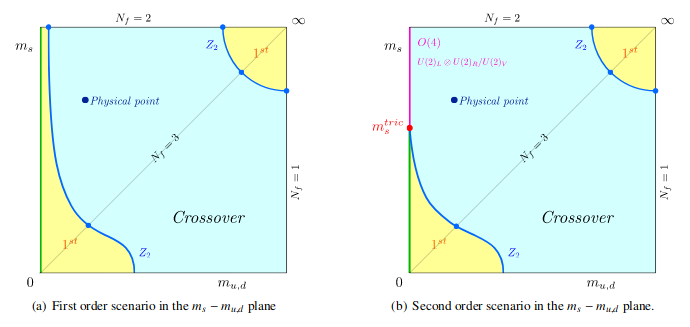
\includegraphics[width=1.0\textwidth]{columbia.png}
\end{minipage}
\hfill
\caption{Two possible scenarios for the Columbia Plot with the up and down quark mass taken to be identical. The ``physical point" is the Standard Model. Plot from \cite{Cuteri:2017zcb}
}
\label{fig:columbia}
\end{figure*}

Beginning with the work of Pedro Schwaller \cite{Schwaller:2015tja} and continuing through the work of many others \cite{everyoneelse}, strong first order phase transitions for SU(N) dark sectors with arbitrary numbers of flavours have been explored as a source of gravitational waves. As $N$naturalness features $N$ distinct QCD sectors, this becomes an incredibly important potential signature of this class of models. Crucially, the behaviour of the QCD phase transition for each sector must be understood --- sectors that feature a weak cross-over transition do not generate the sought after gravitational wave signatures.

Due to the confining nature of QCD, the exact nature of the phase transition is often difficult to ascertain analytically and requires the study of lattice simulations. The results of these studies on the nature of QCD phase transitions is summarized in the so-called ``Columbia" plot (Fig. \ref{fig:columbia}). As seen in the above figure (and explicitly demonstrated through lattice studies \cite{lattice}), our sector is solidly in the weak-cross over area. In order to observe the strong first order transition required for gravitational wave production, at least some of the additional sectors present in $N$naturalness must feature quarks in either the heavy quark (pure Yang-Mills) or massless limits.    

In the Yang-Mills limit we see $m_{u,d,s} \rightarrow \infty$. This leads to the presence of a global $Z_3$ centre symmetry that is broken at high temperatures but restored low temperatures. Ultimately, this restoration results in a first order phase transition \cite{SVETITSKY1982423}. On the other end of the spectrum, ``massless" quark theories ($m_q \ll \Lambda_{QCD}$ for all quarks) also contain strong phase transitions due to the breakdown of SU$(N)\,\times$ SU$(N)$ chiral symmetry \cite{Pisarski:1983ms}. Both the Yang-Mills and massless limit arguments can be generalized to SU$(N \geq 3)$: coupling both with the additional restriction that we avoid the conformal window indicates that strong first order phase transitions can occur if we have $n = 0$ (pure Yang-Mills) or $3 \leq n < 4N$ (light quark limit) very light flavours.

For $N$naturalness, standard sectors with higher vevs possess more massive quarks; eventually, sectors with large enough vevs push us into the upper-right corner. Conversely, exotic sectors with zero vev feature incredibly light quarks and drop us into the bottom-left corner. In order to figure out the specifics of each sector, we follow  the same procedure as \cite{Cui:2011wk} but generalize it to an arbitrary number of additional sectors. First, due to the parameters of each sector being taken to be identical save for the higgs mass squared (thus $v \neq v_i$, where $v$ is the SM vev), we assume that the strong coupling of every sector is identical at some high scale. 
Explicitly, above the top quark mass scale $\Lambda_{QCD} = 89 \pm 5$ in $\overline{MS}$ \cite{PhysRevD.98.030001}. Since the running of the gauge coupling at scale $\mu$ is given by 
\begin{equation}\label{eqn:QCDrunning}
\alpha_s (\mu) = \frac{2\pi}{11-\frac{2n_f}{3}}\frac{1}{\ln{\mu/\Lambda}}
\end{equation} 
where $n_f$ is the number of quark flavours and $\Lambda$ is the confinement scale $\Lambda_{QCD}$ \cite{Peskin:1995ev}. 

For any other sector $i$ we write out the expression as: 
\begin{equation}\label{eqn:QCDrunningi}
\alpha_{s}^i (\mu) = \frac{2\pi}{11-\frac{2n^i_f}{3}}\frac{1}{\ln{\mu/\Lambda^i}},
\end{equation}
featuring the equivalent definitions for the additional sectors. Because we've set the strong couplings equal at high scales, $\Lambda = \Lambda^i$ for all $i$ at scales above the top quark mass for the heaviest sector. However, since the masses of the quarks in each sector are different, we end up with a unique running of the coupling for each sector. At every quark mass threshold for a given sector, we match the coupling strengths above and below the threshold and determine the new $\Lambda^i$ for the lower scale:
\begin{equation}
\alpha_s^{i(5)} = \alpha_s^{i(6)}
\end{equation} 
and thus
\begin{equation}
\Lambda_{(5)}^i = (m_t^{i})^{2/23}(\Lambda_{(6)}^i)^{21/23}.
\end{equation}

Suppressing the $i$s for cleanliness, we can arrive at similar relations at the bottom and charm thresholds
\begin{equation}
\begin{split}
\Lambda_{(4)} = (m_b)^{2/25}(\Lambda_{(5)})^{23/25},
\\
\Lambda_{(3)} = (m_c)^{2/23}(\Lambda_{(4)})^{25/27}.
\end{split}
\end{equation}
These can be combined to show that
\begin{equation}
\Lambda_{(3)} = (m_t m_b m_c)^{2/27}(\Lambda_{(6)})^{21/27}.
\end{equation}
This type of matching procedure can be done as many times as necessary for a given sector. The process terminates when $\Lambda_i$ for a given scale is larger than the next quark mass threshold (i.e running the scale down arrives at the $\Lambda_{QCD}$ phase transition before reaching the next quark mass scale).

In cosmological terms, we can envision a sector's thermal history unfolding where as the plasma cools below each quark mass threshold, said quarks are frozen out. At a certain point, the sector arrives at the QCD phase transition and confinement occurs (provided there are light enough quarks to confine) --- if this occurs when $\geq 3$ quarks are at a much lower scale or all quarks have already frozen out, we get the desired phase transition.   

\subsection{Standard Sectors}

\begin{figure}
\centering
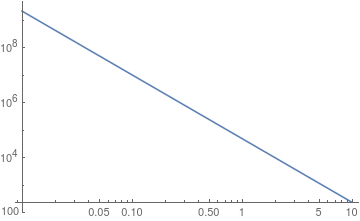
\includegraphics[width=0.45\textwidth]{critIndex.png}

\hfill
\caption{Critical index $i$ as a function of slop factor. 
}
\label{fig:critIndex}
\end{figure}

As mentioned in the previous sections, for standard sectors with increasing index $i$ the vevs of said sectors increase $v_i\propto \sqrt{i}$. This leads to increasingly heavy particle spectra for higher sectors --- eventually leading to sectors that are essentially pure Yang-Mills that featuring strong first order phase transitions. This, of course, begs the question: at what index $i$ do said phase transitions begin?

The actual boundary of region of interest on the Columbia plot is not precisely known and further lattice simulations are required to determine exactly where in parameter space cross-over transitions end and first order transitions begin. In lieu of such studies, we parameterize our ignorance in the form of a ``slop factor" $\kappa$. Assuming the up and down quarks of each sector to be of roughly the same scale, we determine what sector $i$ features $\kappa m_u^i \approx \Lambda_{QCD}$.

Using the methods outlined in the prior section we determine $\Lambda_{QCD}$ to have a relevant value of 
\begin{equation}\label{eqn:lambda2}
\Lambda^i_{(2)} = (m_s^i m_c^i m_b^i m_t^i)^{2/29}(\Lambda^i_{(6)})^{21/29}
\end{equation} 
at the energy scale we're interested in. $\Lambda^i_{(6)}$ is identical for all sectors and is taken to have a standard model value. Rewriting Eq. (\ref{eqn:lambda2}) in terms of standard model variables, 
\begin{equation}\label{eqn:lambda2adj}
\Lambda^i_{(2)} = (m_s m_c m_b m_t i^2)^{2/29}(\Lambda_{(6)})^{21/29}.
\end{equation}
Setting this equal to some multiple of the quark mass of sector $i$,
\begin{equation}
\kappa m^i_u = \kappa m_u \sqrt{i} = (m_s m_c m_b m_t i^2)^{2/29}(\Lambda_{(6)})^{21/29}.
\end{equation}
This can be solved for $i$:
\begin{equation}\label{eqn:critIndex}
i = \frac{(m_s m_c m_b m_t)^{4/25}(\Lambda_{(6)})^{42/25}}{(\kappa m_u)^{58/25}}.
\end{equation}
The results as a function of $\kappa$ are plotted in Fig. \ref{fig:critIndex}. 
 
The critical index plot (Fig. \ref{fig:critIndex}) clearly demonstrates that even in the most extreme cases, where first order phase transitions occur with the up quark an order of magnitude less than $\Lambda_{QCD}$, the critical index is still $\sim 1000$. Looking back to the energy density plot (Fig. \ref{fig:energyDensity}), we see the energy density of these sectors is at most $10^{-8}$ that of our sector. As a result, the gravitational waves generated by the standard large $i$ sectors in $N$naturalness will not generate detectable signatures. 

\subsection{Exotic Sectors}

In every exotic sector the fermion masses are exceptionally light: even the most massive quark of each sector is orders of magnitude smaller than our confinement scale, $m_t \ll \Lambda_{QCD}$. Additionally, since $m_q \propto 1/(m^2_H)_i$ this separation only becomes more pronounced as we move to sectors further from our own. The scale of the exotic quarks makes it unnecessary to run down the scale of the strong coupling as done for the standard sectors --- the phase transition for all exotic sectors occurs at $\sim 90 \,\mathrm{MeV}$ and a strong first order phase transition occurs for all exotic sectors at this temperature. 

The confinement of these sectors directly leads to the production of both baryons and mesons as we have the spontaneous breaking of SU$(6) \,\times$ SU$(6) \rightarrow\,$ SU$(6)$. This leads to the production of 35 pseudo-Goldstone bosons during the phase transition. These become relevant in the calculation of gravitational wave signatures through the calculation of the critical phase transition strength, $\alpha_{\infty}$, with $\alpha_{\infty}$ denotes the dividing line between the runaway regime  $(\alpha >\alpha_{\infty})$ and the non-runaway regime $(\alpha <\alpha_{\infty})$. Explicitly \cite{Breitbach:2018ddu, Caprini:2015zlo, Espinosa:2010hh}, 
\begin{equation}\label{eqn:critPTstrength}
\alpha_{\infty} = \frac{(T^{nuc}_h)^2}{\rho_R}\left[\sum_{bosons} n_i\frac{\Delta m^2_i}{24} + \sum_{fermions} n_i\frac{\Delta m_i^2}{48}\right],
\end{equation} 
for particles with $n_i$ degrees of freedom that obtain mass through the phase transition. 

The masses obtained through the phase transition can be approximated through the use of a generalization of the Gell-Mann--Oakes--Renner relation \cite{Schwartz:2013pla},
\begin{equation}\label{eqn:gmor}
m^2_{\pi} = \frac{V^3}{F^2_{\pi}}(m_u + m_d),
\end{equation}
where $V \sim \Lambda_{QCD}$, $F_\pi$ is the pion decay constant. So, for mesons in exotic sector $i$:
\begin{equation}
m_{\pi}^i \sim \sqrt{\frac{m_1^i+m_2^i}{m_u + m_d}} m_{\pi}.
\end{equation}
Ultimately, calculating the critical phase transition strength for each sector using Eq. (\ref{eqn:critPTstrength}) indicates that every sector has a phase transition in the runaway regime. Thus, all exotic sectors have strong first order phase transitions that lead to runaway bubble walls.

\section{Constraints}
\label{sec:constraints}

\begin{figure}
\centering
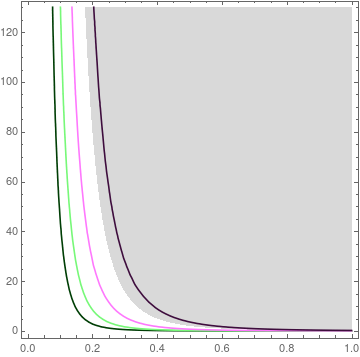
\includegraphics[width=0.45\textwidth]{NeffBounds.png}
\label{fig:Neff}
\hfill
\caption{$\Delta N_{eff}$ as a function of relativistic degrees of freedom in a fully decoupled hidden sector ($g_h$) and the temperature ratio of said sector. Contours set $\Delta N_{eff}$ to 0.01 (forest green), 0.03 (lime green), 0.1 (gentle pink), and 0.5 (royal violet). Most stringent current $N_{eff}$ bounds shade in grey. 
}
\end{figure}

In general, the multi-hidden sector models explored here feature feature of huge number of (nearly) massless degrees of freedom. Dark photons, neutrinos, and the like abound in these sectors and, assuming a relatively high reheat temperature, the leptons, quarks, and baryons of these sectors are can easily be relativistic. In $N$naturalness this feature is realized quite dramatically: each of the thousands (or millions or billions) of sectors possess relativistic degrees of freedom. The presence of these particles can have two main effects: extra relativistic particles can alter the expansion history of the universe through changes to the energy density or hidden sectors can feature annihilations that reheat the photons or neutrinos of our sector near Big Bang Nucleosynthesis (BBN) and affect the light element abundances. The effective number of neutrino species, $N_{eff}$, describes these contributions and, as such, is the strictest constraint that must be dealt with when studying these type of multi-phase transition models. 

The SM predicts that $N^{SM}_{eff} = 3.046$ \cite{Mangano:2005cc}. This is in good agreement with bounds from studies of the Cosmic Microwave Background (CMB) by Planck combined with bayon acoustic oscillations (BAO) measurements \cite{Aghanim:2018eyx}:
\begin{equation}
N_{eff} = 2.99^{+0.34}_{-0.33}.
\end{equation}
Various different assumptions about the history of the universe can be made and different data sets can be chosen to obtain slightly different results \cite{Breitbach:2018ddu} --- for the purposes of this exploratory work, wading through this landscape is unnecessary.

For fully decoupled sectors that never enters (or reenters) thermal equilibrium with our sector, we obtain additional contributions to $N^{SM}_{eff}$ \cite{Breitbach:2018ddu}
\begin{equation}\label{eqn:DeltaNeff1hs}
\Delta N_{eff} = \frac{4}{7}\left(\frac{11}{4}\right)^{4/3}g_h \xi_h^4.
\end{equation} 
Here, $g_h$ represents the effective number of relativistic degrees of freedom for the hidden sector when the hidden sector has a temperature $T_h = \xi_h T_\gamma$. Contours for Eq. (\ref{eqn:DeltaNeff1hs}) at various temperature ratios as well as CMB bounds are plotted in Fig. \ref{fig:Neff}. We take this approach and generalize it to include many additional sectors:
\begin{equation}\label{eqn:DeltaNeff}
\Delta N_{eff} = \sum_i \frac{4}{7}\left(\frac{11}{4}\right)^{4/3}g_{i} \xi^4_{i}.
\end{equation} 

As Fig. \ref{fig:Neff} demonstrates, sectors with a temperature ratio above $\xi_h\sim 0.5$ with even a couple of relativist particles are immediately excluded by CMB constraints. Accordingly, the additional sectors present in this project must be heated to a much smaller fraction of our own sector's temperature. 

\subsection{Exotic Sector Contributions}

The original $N$naturalness paper focused on the (stronger) $N_{eff}$ constraints from the additional standard sectors and ignored the exotic sectors altogether \cite{Arkani-Hamed:2016rle}; in contrast, we take the opposite approach. Since we're more interested in a more general scenario with multiple dark phase transitions, we focus in on whether zero vev sectors can dodge these $N_{eff}$ bounds.

Within the framework of SM-like sectors (save the higgs mass parameter), our exotic sectors feature at most 106.75 effective degrees of freedom at high energies: 72 from quarks,  12 from charged leptons, 6 from neutrinos, 16 from gluons, 2 from photons, 6 from W bosons (no longitudinal modes due to a no symmetry breaking), 4 from the higgs sector (again, no symmetry breaking leads to 3 additional modes), for a total of 118 degress of freedom. Scaling the fermionic contributions by $7/8$ gives us 106.75 effective relativistic degrees of freedom.  After the higgses freeze out, 4 degrees of freedom are lost; when the QCD phase transition occurs 35 bosonic degrees of freedom are gained while 72 fermionic are lost, leaving 56.75 effective degrees of freedom. Since all additional sectors are colder than our own by the time photon decoupling occurs ($\sim 0.39 \ev$), the pions of all of these sectors have a much higher mass in accordance with Eq. (\ref{eqn:gmor}) and thus will have frozen out long before --- leaving at most $11.25$ effective degrees of freedom per sector.

Coupling the number of effective degrees of freedom per sector with the energy density scaling of $\sim 1/m_H^4$ found in the zero vev sectors leads to tiny temperature ratios. Assuming a reheating temperature of $100$ GeV and a completely uniform distribution of sectors, the temperature of the first exotic sector is slightly more than $6\%$ of our sector at reheating. Applying Eq. (\ref{eqn:DeltaNeff}) to this particular situation gives us:
\begin{equation}
\Delta N_{eff} = \sum_i \frac{4}{7}\left(\frac{11}{4}\right)^{4/3}g_{i} \left(\frac{0.06}{i^2}\right)^4.
\end{equation}     
Summing over all sectors (sectors above $i \sim 10$ essentially don't contribute due to the small temperature ratio) gives us a contribution of $\mathcal{O} (10^{-4})$. Evolving the sectors thermal histories forward in time to the recombination era gives us a slightly larger value, but still of order $\mathcal{O}(10^{-4})$; well under current CMB bounds. 

In additional runs completed with various adjustments to the exotic sectors (e.g. adjusting the exotic sectors to have a lower higgs mass squared or clustering multiple hidden sectors close to the first exotic one) the value of $\Delta N_{eff}$ coming from the exotic sectors is larger than the base $N$naturalness case. This increase is, for the most part, not excluded by current bounds, but will be mostly probeable by next generation CMB experiments. 


\section{Signals}
\label{sec:signals}

\section{Conclusion}
\label{sec:conclusion}


%%%%%%%%%%%%%%%%%%%%%%%%%
%%%%%%%%%%%%%%%%%%%%%%%%%
%%%%%%%%%%%%%%%%%%%%%%%%%
%%%%%%%%%%%%%%%%%%%%%%%%%
%%%%%%%%%%%%%%%%%%%%%%%%%
\appendix

%%%%%%%%%%%%%%%%%%%%%%%%%%%%%
\bibliographystyle{apsrev4-2}
\bibliography{refs}

\end{document}





